% siminos/spatiotemp/chapter/Bernoulli.tex
% $Author: predrag $ $Date: 2021-12-20 23:24:25 -0500 (Mon, 20 Dec 2021) $

% called by siminos/spatiotemp/blogCats.tex
\section{Bernoulli map, beta transformation}
\label{sect:Bernoulli}

%\exercise{$\beta$ map}{
%Use single slope map to show how hard life is.
%\PC{find references - Flato?}
%\label{e_beta}
%}

\begin{description}

\item[2021-01-04 Predrag] discussed here:

\toChaosBook{exmple.14.5}{example~{14.5}}
{\em Bernoulli shift map state space partition}

\toChaosBook{equation.27.4.23}
{example~{27.3}} {\em Lyapunov exponents for 1-dimensional maps.}

The (unnumbered) equation, the end of \toChaosBook{section.28.6}
{section~{28.5}} {\em Analyticity of spectral determinants.}

\toChaosBook{exmple.28.5}
{example~{28.2}} {\em Bernoulli shift eigenfunctions.}

\toChaosBook{Item.451}
{exercise~{28.5}} {\em Bernoulli shift on $L$ spaces.}

\toChaosBook{exmple.29.1}
{example~{29.1}} {\em Return times for the Bernoulli map.}

\toChaosBook{section.N.3}
{appendix~{28.5}} {\em Pruned Bernoulli shift.}

See
\refrem{rem:Bernoulli}~{\em Bernoulli map.}
\refrem{rem-GroRue}~{\em Bernoulli shift.}

See discussion around \refeq{1stepDiffEq}.

See \refeq{genFuncts:noPerPtsBm}.

\HREF{https://en.wikipedia.org/wiki/Dyadic_transformation}
{wiki: Dyadic transformation}
also known as the dyadic map, bit shift map,
2x mod 1 map, Bernoulli map, doubling map, sawtooth map.



    \PCpost{2020-01-27}{Dropped:
Much of ergodic theory can be illustrated by a Bernoulli
map\rf{Driebe99,BoyGor97}. One can explicitly construct a \FPoper, and
compute its eigenvalues and its eigenvectors; construct the {\dzeta}, and
count {\lattstate}s and {\orbit}s\rf{ChaosBook}.

 (for  $\shift$ written out as a matrix, see
\refeq{appe:Bern_cyc})
    }


\item[2019-07-30 Predrag]
Since all coefficients in \refeq{OneCat} are integers, the {\lattstate}s
$\ssp_\zeit$  are always rational. This allows for their exact evaluation
by integer arithmetic.

\item[2019-12-18 Predrag] (dropped from \texttt{CL18.tex})\\
Restrict the
admissible field values $\ssp_{t}$ at time-lattice site $t$ to the
symmetric unit interval $\ssp\in[-1/2,1/2)$, with ??-letter alphabet
\beq
\A=\{\underline{4},\underline{3},\underline{2},\underline{1},
     0,1,2,3,4\}
\,.
\ee{SawtoothFace6alph}

It maps the unit
interval onto itself, with fixed points $\ssp_0=0$, $\ssp_1=1$.

reduction
$\hflow{}{\ssp_{\zeit}}\mapsto\flow{}{\ssp_{\zeit}}$

Recall how the subpartitions of \reffig{fig:BernPart} were used to
obtain the total number of periodic points \refeq{noPerPtsBm}, as every
subpartition contained one and only one periodic point.

%
%%%%%%%%%%%%%%%%%%%%%%%%%%%%%%%%%%%%%%%%%%%%%%%%%%%%%%%%%%%%%%%%%%
%\FIG{
\begin{figure}
  \centering
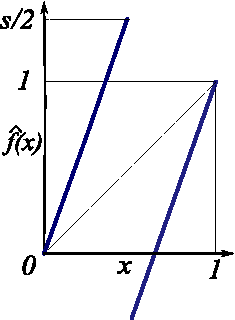
\includegraphics[width=0.30\textwidth]{fig_d_1CL18}
  \caption{\label{fig-d-1f}
$\hflow{}{\ssp}$, the full space sawtooth map \refeq{KD-mapCL18}, ${s} >
2$.
            }
\end{figure}
%%%%%%%%%%%%%%%%%%%%%%%%%%%%%%%%%%%%%%%%%%%%%%%%%%%%%%%%%%%%%%%%%%
%
The closely related {\em sawtooth map}, sketched in \reffig{fig-d-1f},
with `stretching' parameter $s>2$,
\index{sawtooth map}
\beq
\hx_{\zeit+1}
    \,=\, \hflow{}{\hx_{\zeit}}
    \,=\,\left\{
\begin{array}{ll}
{s} \hx_{\zeit}\,,          & \hx_{\zeit} \in [0,{1/2}) \\
{s} \hx_{\zeit} +1 - {s}\,, & \hx_{\zeit} \in ({1/2},1]
\end{array}
\right.
%\,,\qquad {s} \in \{2,3,4, \cdots\}
%\,,
\label{KD-mapCL18}
\eeq

 Since the relation between $\Ssym{\zeit}$ symbol
sequences and $\ssp_{\zeit}$ states is linear, it is straightforward  to
go back and forth between a {\lattstate} and its symbolic
representation.

%%%%%%%%%%%%%%%%%%%%%%%%%%%%%%%%%%%%%%%%%%%%%%%%%%%%%%%%%%%%%
\begin{figure}
  \centering
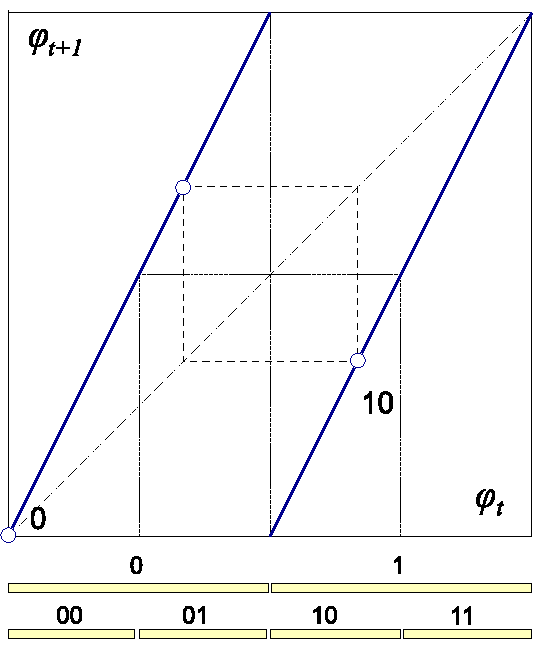
\includegraphics[width=0.35\textwidth]{BernPartKitten}
  \caption{\label{fig:BernPart}
The Bernoulli map \refeq{KD-mapCL18} for ${s}=2$, %{BerShift},
together with the
$\cycle{0}$ fixed point, and the \cycle{01} 2-cycle. Preimages
of the critical point $\ssp_c=1/2$ partition the unit interval into
$\{\pS_0,\pS_1\}$, $\{\pS_{00},\pS_{01},\pS_{10},\pS_{11}\}$, $\dots$,
subintervals.
As the map is a
circle map, $\ssp_{5}=1=0=\ssp_{0} \quad(\mbox{mod}\;1)$.
          }
\end{figure}
%%%%%%%%%%%%%%%%%%%%%%%%%%%%%%%%%%%%%%%%%%%%%%%%%%%%%%%%%%%%%%

The $n$th
preimages $b^{-(n-1)}(\ssp)$ of the critical point $\ssp_c=1/2$
partition the \statesp\ into $2^n$ subintervals, each labeled
by the first $n$ binary digits of points $\ssp=.\Ssym{1}
\Ssym{2} \Ssym{3} \ldots $ within the subinterval:
\reffig{fig:BernPart} illustrates such 4-intervals \statesp\
partition $\{\pS_{00},\pS_{01},\pS_{11},\pS_{10}\}$  for
$\cl{}=2$.

known as the {\em doubling} map if ${s}=2$,
    \index{doubling map}\index{circle map}
\beq
\ssp_{\zeit+1} = 2 \ssp_{\zeit} \;\; (\mbox{mod}\;1)
%    \,,\qquad \qquad \ssp_{\zeit}\in [0,1)
\,,
\ee{DoublingMap}
and {\em ${s}$-tupling} map, \reffig{fig-d-1}\,(b), for
integer stretching parameter ${s}\geq3$,

The relation is linear, and a given \brick\ $\Mm$, or `code' in terms of
alphabet  \refeq{base-sAlph}, corresponds to a unique temporal {\lattstate} $\Xx$ given by the lattice Green's function
\beq
\Xx
= \gd\,\Mm
\,,\qquad
\gd = - \frac{\shift}{\shift - s\,\id}
\,,
\ee{appe:tempBernGreen}
provided we specify the boundary conditions ({\bcs}) for the {\shiftOp}
$\shift$.

The power of the linear encoding of the {temporal
Bernoulli} condition \refeq{1stepDiffEq} is that the
\emph{integer}-valued symbols $\Ssym{\zeit}$ from the finite alphabet
\refeq{base-sAlph} encode the \emph{real-valued} lattice site states
$\ssp_{\zeit}$.

For the  %\rf{GroFuj,art91},
piecewise linear map of \reffig{fig:BernPart}
we can evaluate the \dzeta\ in closed form.
Each branch has the same value of the
slope, and the map can be parameterized
by the single parameter ${s}$.
The larger ${s}$ is, the stronger is the stretching action of the map.

The power of the code % $\{\Ssym{\zeit}\}$
\beq
\transp{\Mm} % = \{\ssp_j\}
             = (\Ssym{\zeit},\Ssym{{\zeit+1}},\cdots,\Ssym{{\zeit+k}})
\ee{linCode}
for the {\templatt} \refeq{OneCat} is that one can use \emph{integers}
$\Ssym{\zeit}$ to encode the \emph{real-valued} {\lattstate}s $\ssp_{\zeit}$.

,
\beq
(\partial - (s-1)\,\shift^{-1})\,\Xx = -\Mm
\,.
\ee{app:1stepVecEq}

For
the $s=3$ cat map example at hand, they are
\beq
\{M_j\} = (M_1,M_2,M_3,M_4,M_5,\cdots)
=(1,2,5,10,24,\cdots)
\,,
\ee{noPrimeCycs=3}

Visualizing the volume relation \refeq{eq:fundFact} for a general \cl{}\dmn\
{\fundPip} is not easy, but

As the {temporal Bernoulli} \refeq{tempBern} is linear, eigenmodes of
$\jMorb$, shifted by $\Mm$ as in \refeq{tempBern} for each distinct
{\lattstate}, are also {\lattstate}s of {temporal Bernoulli}.


    \HLpost{2020-01-17}{
The determinant of this $\jMorb$ from \refeq{tempBern} is negative so
we cannot use the determinant trace formula directly. A correct way is:
first rewrite the $\jMorb$ as in \refeq{appe:tempBernGreen}
\[
\jMorb = \id-{s}{\shift}^{-1}
       = - \frac{s}{\shift} \left(\id-\frac{\shift}{s}\right)
\, .
\]
Note that $\det(\shift)=(-1)^{\cl{}-1}$. The determinant of $\jMorb$ is:
\[
\det \jMorb = \det(\frac{\shift}{s}-\id) s^{\cl{}}(-1)^{\cl{}-1}
   = - s^{\cl{}} \det(\id-\frac{\shift}{s}) \, .
\]
Then use the determinant-trace formula:
\[
\ln\det(\id-\frac{\shift}{s}) = \tr\ln({\id- {\shift}/{s}})
  =
-\sum_{k=1}^\infty\frac{1}{k}\frac{\tr(\shift^k)}{s^k}
\, ,
\]
and use
$\tr \shift^k= \cl{}\delta_{k,\cl{}r}$ if $k$ is a multiple of $\cl{}$,
0 otherwise
(follows from $\shift^\cl{}=\id$),
\[
\ln\det(\id-\frac{\shift}{s}) = -\sum_{r=1}^\infty\frac{1}{r}\frac{1}{s^{\cl{}r}}
=
\ln(1-s^{-\cl{}})
\, ,
\]
and the determinant of $\jMorb$ is:
\[
\det \jMorb = - s^{\cl{}} \det(\id-\frac{\shift}{s}) = 1 - s^{\cl{}}
\, ,
\]
which is negative. So for the {temporal Bernoulli} the count is:
\[
N_\cl{} = |\det \jMorb| = s^{\cl{}} - 1
\, ,
\]
in agreement with the time-evolution count \refeq{noPerPtsBm}.
}

\item[2020-01-25 Predrag:] {\bf A Bernoulli map example}.
%%%%%%%%%%%%%%%%%%%%%%%%%%%%%%%%%%%%%%%%%%%%%%%%%%%%%%%%%%%%%%%%%%%%%%%
% BernCyc2Jacob.svg
% derived from CatMapStatesp.svg
\begin{figure}
  \centering
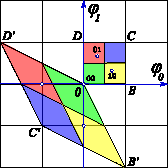
\includegraphics[width=0.45\textwidth]{BernCyc2Jacob}
  \caption{\label{fig:BernCyc2Jacob}
(2020-02-14 Predrag: his is ``wrong'', now superseded with the updated
figure in \refref{CL18}; 2020-09-11 the whole example seems misplaced
here, moce it to wherever it belongs)
The base-2 Bernoulli map \refeq{circ-m=2} period-2 periodic points
$\Xx_p=(\field_0,\field_1)$ are $\cycle{0}=(0,0)$, $\cycle{1}=(1,1)$ fixed
point repeats, and the 2-cycle $\Xx_{01}=({1}/{3},{2}/{3})$,
see \reffig{fig:BernPart}.
They all lie within the unit square $[0BCD]$, one within each
$\pS_{\Ssym{0}\Ssym{1}}$ subregion, and are mapped by the
$[2\!\times\!2]$ {\jacobianOrb} $\jMorb$
% \refeq{jacobianOrb}
into the parallelogram $[0B'C'D']$, whose area is 4 times the unit area.
The images of periodic points $\Xx_p$ land on the integer lattice, and
are sent back into the origin by integer translations $\Mm_p$, in order
to satisfy the fixed point condition
%\refeq{tempBernFix},
$\jMorb\Xx_p+\Mm_p=0$.
          }
\end{figure}
%%%%%%%%%%%%%%%%%%%%%%%%%%%%%%%%%%%%%%%%%%%%%%%%%%%%%%%%%%%%%%
%
The action of {\jacobianOrb}
$\jMorb$ for the period-2 periodic points of the base-2 Bernoulli map,
\reffig{fig:BernPart},
which partitions the unit interval into ${2}$ subintervals
$\{\pS_\Ssym{}\}$, is
\beq
\field_{\zeit+1}
= {2} \field_{\zeit} - \Ssym{\zeit+1}
\,,\qquad  \field_{\zeit}\in\pS_{\Ssym{\zeit}}
\,,
\ee{circ-m=2}
where $\Ssym{\zeit}$ takes values in the ${2}$-letter alphabet
\beq
\Ssym{} \in \A=\{0,1\}
\,.
\ee{base-sAlph=2}

should suffice to convey the idea. In this
case, the $[2\!\times\!2]$ {\jacobianOrb}, the unit
square basis vectors, and their images are
\bea
\jMorb &=&
 \left(\begin{array}{cc}
  1 & -2 \\
 -2 &  1
 \end{array} \right)
;\quad
\Xx_B =
 \left(\begin{array}{c}
 1  \\
 0
 \end{array} \right)
\,,\quad
\Xx_D =
 \left(\begin{array}{c}
 0  \\
 1
 \end{array} \right)
\continue
\Xx_{B'}  &=& \jMorb\,\Xx_B =
 \left(\begin{array}{c}
  1  \\
 -2
 \end{array} \right)
\,,\quad
\Xx_{D'} =
 \left(\begin{array}{c}
-2  \\
 1
 \end{array} \right)
\,,
\eea
with the resulting fundamental parallelogram of area 4
shown in \reffig{fig:BernCyc2Jacob}.
The volume of the fundamental parallelogram lattice $\lattice$ \refeq{lattVol} is
\beq
\Det(\lattice) = \Det(\Xx_{B'}|\Xx_{D'})= \Det(\jMorb)\,\Det(\Xx_{B}|\Xx_{D}) = - 3
\,,
\ee{bernVol}
where in this case the unit cell matrix $(\Xx_{B}|\Xx_{D})=\unit$.


The $[3\!\times\!3]$ {\jacobianOrb} and the unit
cube basis vectors are
\bea
- \jMorb &=&
 \left(\begin{array}{ccc}
  -1  & 0 & 2 \\
  2 &  -1 & 0\\
  0 & 2 & -1
 \end{array} \right)
\,,\quad
\left(\Xx_B|\Xx_C|\Xx_D\right) =
 \left(\begin{array}{ccc}
 1 & 0 & 0\\
 0 & 1 & 0\\
 0 & 0 & 1
 \end{array} \right)
\,.
\nnu
\eea
Clearly $\Det(-\jMorb)= {s}^3-1$, and so on, reproducing the periodic
states count for Bernoulli. No point of looking at $\Det(-\jMorb)$, as
that changes sign at every order - always evaluate $|\Det(\jMorb)|$.

%%%%%%%%%%%%%%%%%%%%%%%%%%%%%%%%%%%%%%%%%%%%%%%%%%%%%%%%%%%%%%%%%%%%%%%
% BernCyc2Jacob.svg
% derived from CatMapStatesp.svg
\begin{figure}
  \centering
{(a)}
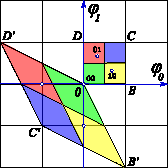
\includegraphics[width=0.35\textwidth]{BernCyc2Jacob}
~~~
{(b)} %$\!\!\!\!$
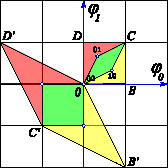
\includegraphics[width=0.35\textwidth]{BernCyc2JacobUnit}
  \caption{\label{fig:BernCyc2JacobOld}
[OLD VERSION] The Bernoulli map \refeq{BerShift} period-2 {\lattstate}s
$\Xx_\Mm=(\ssp_0,\ssp_1)$ are the $\cycle{0}=(0,0)$ fixed
point, and the 2-cycle $\Xx_{01}=({1}/{3},{2}/{3})$, see
\reffig{fig:BernPart}. They all lie within the unit square $[0BCD]$,
one within each $\pS_{\Ssym{0}\Ssym{1}}$ subregion, and are mapped by the
$[2\!\times\!2]$ {\jacobianOrb} $\jMorb$ \refeq{bernFundPar} into the
{\fundPip} $[0B'C'D']$. The images
of periodic points $\Xx_\Mm$ land on the integer lattice, and are sent back
into the origin by integer translations $\Mm$, in order to satisfy the
fixed point condition refeq\{tempFixPoint\}, $\jMorb\Xx_\Mm+\Mm=0$.
\refFig{fig:BernPart} suggests subdividing the {\fundPip}
into (a) 4 areas, but they are not unit areas. The theory of integer lattices
dictates instead (b) covering the {\fundPip} by 3 unit area
rectangles, with
all vertices on the integer lattice.
          }
\end{figure}
%%%%%%%%%%%%%%%%%%%%%%%%%%%%%%%%%%%%%%%%%%%%%%%%%%%%%%%%%%%%%%
%

\PCpost{2020-02-16}{
Dropped from CL18\rf{CL18}:\\
The temporal Bernoulli lattice Green's function %\refeq{appe:tempBernGreen}
in the matrix form
\beq
\gd
=  \left(\begin{array}{ccccccc}
0&\ExpaEig^{-1}&\ExpaEig^{-2}&\ExpaEig^{-3}&\ExpaEig^{-4}&\ExpaEig^{-5}&\cdots\cr
0&  0          & \ExpaEig^{-1}&\ExpaEig^{-2}&\ExpaEig^{-3}&\ExpaEig^{-4}&\cdots\cr
0&  0          &   0          &\ExpaEig^{-1}&\ExpaEig^{-2}&\ExpaEig^{-3}&\cdots\cr
0&  0          &   0          &     0       & \ddots      &  \cr
0&  0          &   0          &     0       & 0           & \ExpaEig^{-1}&\cdots\cr
0&  0          &   0          &     0       & 0           & 0            &\ddots\cr
\vdots&\vdots  &   \vdots     &     \vdots  & \vdots      & \vdots        &\ddots
          \end{array} \right)
\,,
\ee{BernGreenMatrix}
for an infinite temporal Bernoulli
lattice $\zeit\in\integers$, where $\ExpaEig={s}$ is the 1-time step stability
multiplier for the Bernoulli system.
}

\item[2020-02-18 Predrag] Clipped here from
\emph{Ising.tex}, might be relevant to generalizing
Bernoulli to 2\dmn\ lattice, as a warm-up to \catlatt\ zeta functions:

Roettger\rf{Roettger05},
{\em Periodic points classify a family of Markov shifts}, writes:

Ledrappier introduced the following type of space of doubly indexed
sequences over a finite abelian group G,
\[
X_G=\{(x_{s,t}) \in G^{\integers^2} | x_{s,t+1}=x_{s,t}+x_{s+1,t}
\quad \mbox{for all }s,t\in \integers\}.
\]
The group $\integers^2$ acts naturally on the space $X_G$ via left and
upward shifts.

\item[2020-02-19 Predrag]
Suarez\rf{Suarez89}
{\em Difference equations and a principle of double induction},
\CBlibrary{Suarez89}
studies this as a ``partial difference equations,'' that is, difference
equations in two or more variables. He refers to many books on the
subject. His example is a first order hyperbolic equation, with initial
conditions on space and time axes, which describes some thermal
properties,
\[
f(r, m) =f(r, m-1) +f(r-1, m).
%\label{Suarez89(9)}
\]
The goal is to calculate, step by step, all the values of the temperature
T(m,n), starting with the initial and boundary conditions. But then I do
not get the rest of the papers. Perhaps best not to use much time on
`\spt' Bernoulli.

    \item[2020-03-28 Predrag]
The Bernoulli % equation \refeq{circ-m}
first-order difference equation
\beq
\field_{\zeit} - {s}\field_{\zeit-1} = - \Ssym{\zeit}
\,,\qquad  \field_{\zeit} \in [0,1)
\,,
\ee{diffEqs:1stepDiffEq}
{characteristic equation} (for \Ssym{\zeit}=0)
\beq
\ExpaEig -s= 0
\,,
\ee{diffEqs:tempBern}
has one characteristic root
\(
\{s\}
\,.
\)

Comparing with \refeq{genFuncts:noPerPtsBms} we see that we need to solve
a first-order inhomogeneous difference equation with a constant forcing
term $(s-1)$.

Weijie Chen does this pedagogically in his 2011 lecture notes
\CBlibrary{Chen11}, sect.~{\em 1.2.1 One Example}, where he
considers
\beq
\field_{\zeit} - {s}\field_{\zeit-1} = {M}
\,,
\ee{Chen11:1stepDiffEq}
and finds the particular solution by taking
$\field_{p,n} = \field_{p}$ for all $n$,
\[
  \field_{p}-s\,\field_{p}={M}
  \quad \to \quad
  \field_{p} = -{M}/(s-1)
\,.
\]
Hence the solution is
\beq
\field_{n} = \field_{c,n} + \field_{p,n}
= c\,s^{n} - \frac{{M}}{s-1}
\,,
\ee{Chen11:1stepDiffSolu}
with $c$ determined by the initial value
\(
\field_{0}= c\,{s}^{0} - {{M}}/(s-1)
\,.
\)
Bernoulli starts with $\field_{0}=0$, and according to
\refeq{genFuncts:noPerPtsBms}, $M=(s-1)$, so $c=1$.

Weijie Chen also works out the particular solution when $s=1$.
                                    \toCB
He also remarks that in econometrics the {\shiftOp} $\shift$ is called
the \emph{lag operator}.

%\item[2020-03-28 Predrag]
Weijie Chen solves the \templatt\ pedagogically in his lecture notes
\CBlibrary{Chen11}, sect.~{\em 2 Second-Order Difference Equation}.

Questions
\begin{itemize}
  \item
Why is it OK to take site-independent particular solution?
  \item
${{M}}/(s-1)$ looks awkward, can one reformulate? so instead of $M$, have
${{M}}/(s-1)\to1$
  \item
I am guessing that $M=(s-1)$ in \refeq{Chen11:1stepDiffEq}
something like the total number of `letters' I can add to
the count $N_n$ at time $n$. Something like that.
  \item
Similarly for $M=2{\mu}^2$ forcing term in \templatt\ second-order
difference equation \refeq{genFuncts:CatRec-s}.
  \item
This is still just a verification of my guess recurrence
\refeq{genFuncts:noPerPtsBms}.
Make this argument into a derivation.
\end{itemize}

    \PCpost{2020-02-23}{
Just curious - what does the Bernoulli {\fundPip} defined by the columns
of $[3\!\times\!3]$ {\jacobianOrb}
\beq
\jMorb =
\left(
\begin{array}{ccc}
  1 & -2 &  0 \\
  0 &  1 & -2 \\
  -2&  0 &  1
\end{array}
\right)
\,,
\qquad
N_3 = |\Det \jMorb|
    = 2^3-1
\,,
\label{bernFundPar3}
\eeq
look like in a 3\dmn\ rendition? Hopefully it is not symmetric, like
\reffig{fig:catCycJacob}\,(b).
    }

\item[2020-03-01 Predrag]
Wilf\rf{Wilf94} {\em Generatingfunctionology} starts out in his sect.
1.1~{\em An easy 2-term recurrence}, with our Bernoulli periodic points
count \refeq{genFuncts:noPerPtsBm} and
\refeq{genFuncts:1stepDiffEq} as a trivial example of a two-term
recurrence (first-order difference equation).

\item[2020-12-21 Predrag]
{\bf Counting {temporal Bernoulli} {\lattstate}s}
%\label{s:bernCount}
removed from CL18.tex $\to$ Bernoulli.tex, replaced by  refsect{s:Hill1stOrd}
\bigskip

To evaluate the {\HillDet} \refeq{eq:fundFact}, observe that
from \refeq{tempBern} it follows that
\[
\Det(-\jMorb)=\Det({s}/\shift)\,\Det(\id- {\shift}/{s})
\,,
\]
where $|\Det({s}/\shift)|=s^n$. Expand $\ln\Det(\id- {\shift}/{s}) =
\Tr\ln(\id- {\shift}/{s})$ as a series in $1/s$,
\beq
\Tr\ln\left(\id- \frac{\shift}{s}\right)
  =
-\sum_{k=1}^\infty\frac{1}{k}\frac{\Tr(\shift^k)}{s^k}
\,.
\ee{LnDet=TrLn}
It follows from $\shift^\cl{}=\id$ that
$\Tr \shift^k= \cl{}\delta_{k,r\cl{}}$ is non-vanishing
if $k$ is a multiple of $\cl{}$,
0 otherwise:
\[
\ln\Det(\id- {\shift}/{s})
  =
-\sum_{r=1}^\infty\frac{1}{r}\frac{1}{{s}^{\cl{}r}}
  =
\ln(1-{s}^{-\cl{}})
\,.
\]

\item[2020-12-09 Predrag]
{\bf Temporal Bernoulli}
% \label{appe:1D1dLatt}
% was file siminos/kittens/appeBernoulli.tex      pdflatex CL18
%\renewcommand{\statesp}{state space}
%\renewcommand{\Statesp}{State space}
%\renewcommand{\stateDsp}{state-space}
%\renewcommand{\StateDsp}{State-space}
\index{cyclic!permutation matrix}

After $\cl{}$ shifts, the {\lattstate} \Xx\ returns to the initial
state, $\shift^\cl{}=\id$. This relation leads to the explicit expression for
the orbit {\jacobianM} \refeq{appe:tempBernGreen},
\beq
\gd
    =  \frac{\shift}{s\,\id-\shift}
    = \frac{1}{\id-\frac{\shift}{s}}\,\frac{\shift}{s}
    = \sum_{k=1}^\infty \frac{\shift^k}{s^k}
%    =  \sum_{m=0}^\infty \frac{1}{s^{\cl{}m}}
%      \sum_{k=1}^\cl{} \frac{\shift^k}{s^k}
    =  \frac{s^\cl{}}{s^\cl{} - 1}
      \sum_{k=1}^\cl{} \frac{\shift^k}{s^k}
\,.
\ee{appe:BernGreenFct}
From \refeq{appe:tempBernGreen} it then follows that the last field in
$\Xx$ is the field at lattice site $\cl{}$
\beq
\ssp_{\cl{}}
=  \frac{s^\cl{}}{s^\cl{} - 1}
          .\Ssym{1}\Ssym{2}\Ssym{3}\cdots\Ssym{\cl{}}
=  \frac{1}{s - 1}\,%\sum_{k=1}^\cl{} \Ssym{k} 2^{\cl{}-k}
    \frac{s^{\cl{}-1}\Ssym{1}+\cdots+s\,\Ssym{\cl{}-1}+\Ssym{\cl{}}}
         {s^{\cl{}-1}+\cdots+s+1}
\,,
\label{appe:Bern_cyc}
\eeq
and the rest are obtained by cyclic permutations of $\Mm$.

% from ChaosBook \Chapter{appendKnead}
% \section{Pruned Bernoulli shift} \label{sect:PrunBernoulli}
For example, for ${s}=2$, the lattice fields are (they are always rational-valued),
\bea
\ssp_{\Ssym{1}\Ssym{2}\cdots \Ssym{n}}
&=&  \sum_{k=1}^\cl{} \frac{\Ssym{k}}{2^k} \sum_{m=0}^\infty \frac{1}{2^{\cl{}m}}
        = \frac{2^\cl{}}{2^\cl{} - 1} .\Ssym{1}\Ssym{2}\cdots \Ssym{\cl{}}
\continue
&=& \frac{1}{2^\cl{} - 1}\,\sum_{k=1}^\cl{} \Ssym{k} 2^{\cl{}-k}
\,,
\label{Bern_cyc1}
\eea
where $p=\overline{\Ssym{1}\Ssym{2}\cdots \Ssym{\cl{}}}$ is an {\orbit} of period
\cl{}, with stability multiplier $\ExpaEig_p=2^\cl{}$.

For a Bernoulli map,
the rational $\ssp_{0}$ are either periodic or land eventually on a \po\
(the base-${s}$ version of the familiar fact that the decimal expansion
of a rational number is eventually periodic), while the orbit of a normal
irrational $\ssp_{0}$ is ergodic.

    \item[2020-12-09, 2020-12-11 Predrag]
Quotienting the temporal Bernoulli system
\beq
\ssp_{\zeit} - {s}\ssp_{\zeit-1} = - \Ssym{\zeit}
\,,\qquad  \ssp_{\zeit} \in [0,1)
\,,
\ee{1stepDiffEqBlog}
by its \emph{dynamical} $\Dn{1}=\{e,\Refl\}$
symmetry
\beq
\Refl \ssp_\zeit = 1-\ssp_\zeit
    \,,\quad
\Refl \Ssym{\zeit} = (s-1)-\Ssym{\zeit}
    \,,\qquad
\mbox{ for all } \zeit\in\integers
\,,
\ee{BernDynD1}
where $\Ssym{\zeit}$ takes values in the ${s}$-letter alphabet
\beq
\Ssym{} \in \A=\{0,1,2,\cdots,s-1\}
\,.
\ee{base-sAlphBlog}
Define the fundamental domain to be ${\sspRed}_\zeit\in[0,1/2]$.
We construct the
Bernoulli fundamental domain lattice system, with `1/2' unit hypercube
$\hat{\Xx}\in[0,1/2]^\cl{}$, as in
\toChaosBook{exmple.11.3}
{{\em Group \Dn{1} and reduction to the fundamental domain}},
see \reffig{fig:fig_d_2half}\,(b),
and the fundamental domain symbolic dynamics $\hat{\A}$.
The temporal lattice Bernoulli condition \refeq{1stepDiffEqBlog} is now
two conditions  (Bernoulli)/$\Dn{1}$.
They are different for ${s}$ even or odd:
\bea
{\sspRed}_{\zeit+1} - {s} {\sspRed}_{\zeit} &=&
            - \Ssym{\zeit+1}
\,,\qquad  {\sspRed}_{\zeit}\in\pS_{\Ssym{\zeit}}
\,,\quad {s} \mbox{ even}
    \continue
{\sspRed}_{\zeit+1} + {s}{\sspRed}_{\zeit} &=&
       1 + \Ssym{\zeit+1}
\,,\qquad  {\sspRed}_{\zeit}\in\pS_{\Refl\Ssym{\zeit}}
    \label{circ/D1}\\
% \hat{\Ssym{}} \in
\hat{\A}~~~~ &=& \{\{\Ssym{}\},\{\Refl\Ssym{}\}\}
\,,\;\; \{\Ssym{}\} = \{0,1,2,\cdots,{s}/2\}
\,,
\nnu
\eea

\bea
{\sspRed}_{\zeit+1} - {s} {\sspRed}_{\zeit} &=&
\,,\;\;    {s} \mbox{ odd}
\label{base-sRed}\\
%\hat{\Ssym{}} \in
\hat{\A} &=&
\{\{\Ssym{}\},({s}-1)/2,\{\Refl\Ssym{}\}\}
\,,\;\;     \Ssym{}\in \{0,1,2,\cdots,(s-3)/2\}
\,.
\nnu
\eea
As an example, case
${s}=6$,
$\Ssym{\zeit}\in\{0,1,2\}$
is worked out in \reffig{fig:fig_d_2half}\,(c).
(Plot also the fundamental domain map for odd values of ${s}$.)
%
%%%%%%%%%%%%%%%%%%%%%%%%%%%%%%%%%%%%%%%%%%%%%%%%%%%%%%%%%%%%%
\begin{figure}
  \centering
{(a)}
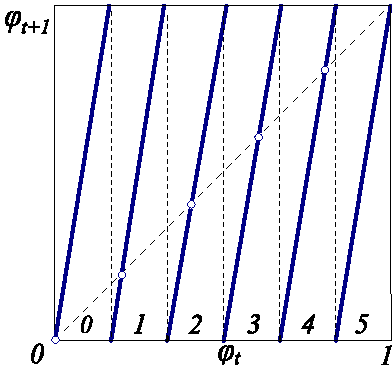
\includegraphics[width=0.40\textwidth]{fig_d_2kitten}
~~~
{(b)}$\!\!\!\!$
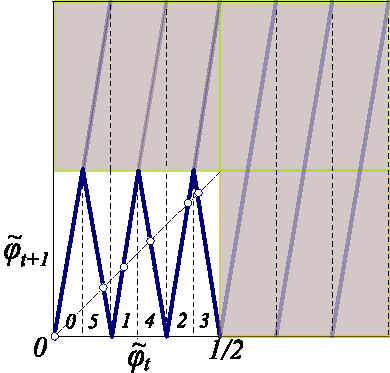
\includegraphics[width=0.40\textwidth]{fig_d_2half}
\\ %~~~
{(c)}$\!\!\!\!$
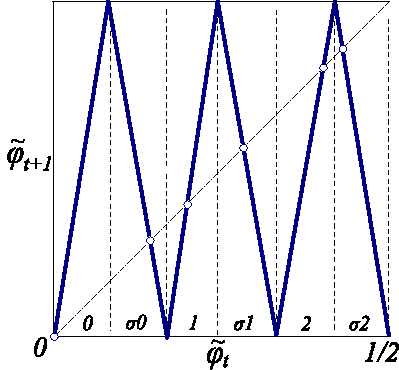
\includegraphics[width=0.40\textwidth]{fig_d_2fund}

  \caption{\label{fig:fig_d_2half}
(a)
The Bernoulli map $f$ with the  stretching parameter ${s}=6$
partitions the unit interval into $6$ subintervals $\{\pS_{\Ssym{}}\}$,
labeled by the ${6}$-letter alphabet \refeq{base-sAlphBlog}. As the map is a
circle map, $\ssp_{5}=1=0=\ssp_{0} \quad(\mbox{mod}\;1)$.
(b)
The Bernoulli map is quotiented by the
\emph{dynamical} $\Group=\Dn{1}=\{e,\Refl\}$
symmetry to
(c)
the fundamental domain ${\sspRed}_\zeit\in[0,1/2]$ map
$\hat{f}=f/\Group$ partitions the half interval into the three $1/12$
subintervals $\{\pS_{0},\pS_{1},\pS_{2}\}$, and their reflections, the
three $3$ subintervals $\{\pS_{\Refl0},\pS_{\Refl1},\pS_{\Refl2}\}$,
labeled by a ${6}$-letter reduced system's alphabet. Reduced space
fixed points $\{\cycle{\Refl_0},\cycle{\Refl_1},\cycle{\Refl_2}\}$
correspond to self-dual 2-cycles
$\{\cycle{05},\cycle{14},\cycle{23}\}$
in the full space. Fixed point $\cycle{0}$ is in the border,
and thus over-counted;
$\cycle{1}$ corresponds to $\{\cycle{1},\cycle{4}\}$, and
$\cycle{2}$ corresponds to $\{\cycle{2},\cycle{3}\}$.
          }
\end{figure}
%%%%%%%%%%%%%%%%%%%%%%%%%%%%%%%%%%%%%%%%%%%%%%%%%%%%%%%%%%%%%%
%

In the matrix form \refeq{1stepDiffEqBlog}, the {\jacobianOrb}
\beq
\jMorb\,\Xx = - \Mm
\,,\qquad
\jMorb = \unit-{s}{\shift}^{-1}
% former \ee{tempBernFix}
\,,
\ee{HLtempBern}
is independent of $\Mm$. Not so for the symmetry reduced  {\jacobianOrb}
${\MvarRed}_{\hat{\Mm}}$ in \refeq{circ/D1}: it depends on
$\hat{\Mm}$, as its diagonal takes values $\pm{s}$. We need to prove
that the \HillDet\ $\Det{\MvarRed}$ does not.

I had not noticed before that this parametrization converts
Bernoulli into tent map, with full \statesp\ 2-cycles turned
into negative slope fixed points.

By the
inclusion-exclusion principle \refeq{KlaRot97(2.1)}
\beq
N_\cl{}=
  \hat{N}_\cl{}+\Refl\hat{N}_\cl{}-\hat{N}_\cl{}\cap(\Refl\hat{N}_\cl{})
      =
  2\hat{N}_\cl{}-\hat{N}_\cl{}\cap(\Refl\hat{N}_\cl{})
\,.
\ee{Bern:inclExcl}
Let's call the number of points in the shared boundary $I$.
% Looks like we have to distinguish odd and even $\cl{}$.
The $\ssp=0$ is in $I$
for any $\cl{}$, if I am allowed to identify $\ssp=1\to0$,
and that is the only point in the boundary.
Presumably this leads to the denominator $(1-z)$ in
\refeq{appe:BernZeta}. I guess that the symmetric irrep of
$\Dn{1}=\{e,\Refl\}$ leads to $N_{+}=s^\cl{}$ and the numerator
$(1-{s}z)$, while the antisymmetric irrep leads to $N_{-}=0$, and a
trivial factor 1 contribution to the numerator \refeq{appe:BernZeta}.
\bea
\zetatop(z)
 &=&
\frac{1 -  {s}z}{1 - z}
\,.
\label{appe:BernZeta}
\eea

\tempLatt\ should be more interesting. Also any nonlinear $s$-branch map
`Bernoulli-like' lattice with a \emph{dynamical} $\Dn{1}$ symmetry; then
the weights $t_p$ do not necessarily cancel for the antisymmetric irrep.

\item[2018-12-27 Linas Vepstas]
{\em On the Beta Transformation} \arXiv{1812.10593}:
The beta transformation is the iterated map \refeq{betaTransf}. The
$\beta=2$ is known as the Bernoulli map, and is exactly solvable. The Bernoulli
map provides a model for pure, unrestrained chaotic (ergodic) behavior:
it is the full invariant shift on the Cantor space. The beta
transformation defines a subshift: iterated on the unit interval, it
singles out a subspace of the Cantor space, in such a way that it is
invariant under the action of the left-shift operator. That is, lopping
off one bit at a time gives back the same subspace. The beta transform
seems to capture something basic about the multiplication of two real
numbers: $\beta$ and $x$. It offers a window into understanding the nature of
multiplication. Iterating on multiplication, one would get
exponentiation; although the mod 1 of the beta transform contorts this in
interesting ways. The work presented here is a research diary: a pastiche
of observations and some shallow insights.
 The eigenvalues of the
transfer operator seem to lie on a circle of radius $1/\beta$ in the complex
plane. Given that the transfer operator is purely real, the appearance of
such a quasi-unitary spectrum seems surprising. The spectrum appears to
be the limit of a dense set of quasi-cyclotomic polynomials, the positive
real roots of which include the Golden and silver ratios, the Pisot
numbers, the n-bonnaci (tribonacci, tetranacci, etc.) numbers.

Beta transformation
\beq
T_{\beta }(x)=\beta x\;{\mod {1}}
\,,\qquad 1<\beta\leq2
\ee{betaTransf}
was introduced by Alfr{\'e}d R{\'e}nyi\rf{Renyi57} in 1957, and an invariant measure for
it was given by Alexander Gelfond in 1959 and independently by Bill
Parry\rf{Parry60} in 1960.

\HREF{https://arxiv.org/pdf/1812.10593.pdf\#subsection.1.9}
{Beta transformation literature review and references}.

\HREF{https://mathoverflow.net/questions/265916/concise-introduction-to-beta-transformations}
{{\em A concise intro to beta-transformations?}} has references.

% A. O. Gel’fand, “A common property of number systems”,
%           Izv Akad Nauk SSSR Ser Mat, 23, 1959, pp. 809–814.

% P. Gaspard, "r-adic one-dimensional maps and the Euler summation
%           formula", Journal of Physics A, 25 (letter) L483-L485 (1992).


\item[2020-09-08 Predrag]
\HREF{https://sites.google.com/site/homepagebingli}{Bing Li}
{\em Some fractal problems in beta-expansions}
\HREF{https://www.irif.fr/~numeration/OWNS}{(video)}
\HREF{https://www.irif.fr/~numeration/uploads/Main/li_20200908.pdf}{(slides)}

For greedy beta-expansions, we study some fractal sets of real numbers
whose orbits under beta-transformation share some common properties. For
example, the partial sum of the greedy beta-expansion converges with the
same order, the orbit is not dense, the orbit is always far from that of
another point etc. The usual tool is to approximate the
beta-transformation dynamical system by Markov subsystems. We also
discuss the similar problems for intermediate beta-expansions.

\item[2021-01-05 Predrag]
Hofbauer and Keller\rf{HofKel84} {\em Zeta-functions and
transfer-operators for piecewise linear transformations} (1984) has no
Bernoulli zeta. Not useful to us at this time.

\item[2021-01-05 Predrag]
Takahashi\rf{Takahashi81} {\em Fredholm determinant of unimodal linear
maps} has lots of detail and examples. I might have missed something, but
Bernoulli zeta is not there, or anything we care about.

\item[2021-01-04 Predrag]
Flatto, Lagarias and Poonen\rf{FlLaPo94}
{\em The zeta function of the beta transformation} (1994)

which should have the $\beta=2$ Bernoulli zeta function
as the trivial case.

\item[2021-01-05 Han] Notes from Flatto, Lagarias and Poonen\rf{FlLaPo94} paper:

$\beta$-transformation map is:
\[
f_\beta(x) = \beta x \;\; (\mbox{mod}\;1) \, ,
\]
where $\beta>1$, $x \in [0,1]$. The symbolic dynamics of $f_\beta$ is based on the fact that the graph of
$f_\beta$ consists of $\lfloor \beta \rfloor + 1$ monotone pieces which they call laps, which are
assigned by the symbols $0, 1, \dots, \lfloor \beta \rfloor$. When $\beta \in \mathbb{Z}^+$,
the piece $\lfloor \beta \rfloor$ consists of a single point, and the symbol $\lfloor \beta \rfloor$
only appears in the itinerary of 1. To each $x \in [1,0]$ its itinerary is $I_\beta(x)=A_0A_1A_2\dots$,
where the symbol
\[
A_n := A_n(x) = \lfloor \beta f_\beta^n(x) \rfloor \, .
\]
In particular the itinerary of 1, $I_\beta(1)=A^*_0A^*_1A^*_2\dots$ encodes complete information about
the behavior of $f_\beta$.

They introduced a power series with integer coefficients:
\[
\phi_\beta(z) = A_0^* z + A_1^* z^2 + A_2^* z^3+ \dots = \sum_{n=0}^{\infty} A_n^* z^{n+1} \, .
\]
This function is related to the iterates of 1 by:
\[
\phi_\beta(z) = 1 + (\beta z - 1)\left(
\sum_{n=0}^\infty f_\beta^n(1)z^n
\right)
\, .
\]
Then the zeta function is:
\[
\zeta_\beta(z) = \frac{1}{1-\phi_\beta(z)} \, ,
\]
if $\beta$ is not a simple $\beta$-number, and
\[
\zeta_\beta(z) = \frac{1-z^N}{1-\phi_\beta(z)} \, ,
\]
if $\beta$ is a simple $\beta$-number, and $N$ is minimal with $f_\beta^N(1)=0$.
Simple $\beta$-numbers are the $\beta$-numbers such that for some $n$, $f_\beta^n(1)=0$.
This formula gives the correct topological zeta function of temporal Bernoulli.

Associated with the $\beta$-transformation is the set $X_\beta$ of all $I_\beta(x)$ for $0 \leq x <1$.
The $\beta$-shift $S_\beta$ is a symbolic dynamical system obtained as the smallest closed (two-sided)
subshift of $\{1,2,\dots \lfloor \beta \rfloor\}^{\mathbb{Z}}$ generated by all finite substrings of $X_\beta$.
For simple $\beta$-numbers $S_\beta$ is a subshift of finite type.

There is a zeta function associated to the $\beta$-shift $S_\beta$, which is studied by
Takahashi\rf{Takahashi83}, who showed that
\[
\hat{\zeta}_\beta(z) = \frac{1}{1-\phi_\beta(z)} \, .
\]
This formula is closely related to $\zeta_\beta(z)$ but differs from it for simple $\beta$-numbers,
in which case the closure operation defining $S_\beta$ adds some extra periodic points.

\item[2021-01-11 Predrag] Seth Lloyd \etal. %\rf{LDGKLMTP20}
{\em Quantum algorithm for nonlinear differential equations}
\arXiv{2011.06571}:

[1] showed how to map the problem of solving a general linear differential
equation to that of matrix inversion, which can then be performed using
the quantum linear systems algorithm [12-13].   Consider a linear differential
equation of the form,
$$ {dx\over dt} + A x = b(t), \eqno(6)$$
where as above $x,b \in {\cal C}^d$ and $A$ is a $[d\times d]$ matrix.

                                                            \toCB
Discretize the equation in time at intervals $\Delta t$, and take $k$ to
be the index for the discretized time, so that $x_k$ and $b_k$ are
the values of $x$ and $b$ at time label $k$.

We wish to integrate equation
(6) numerically starting from the initial state $x_0 \equiv b_0$.   We obtain
a series of equations of the form:
$$
 x_0 = b_0 \quad
x_1 = x_0 - \Delta t A x_0 + \Delta t b_1 \quad
\ldots \quad
x_{k+1} = x_k - \Delta t A x_k + \Delta t  b_k \quad
\ldots
\eqno(7)$$
Here, we have used the Euler forward method for numerical integration, but it
is straightforward to implement implicit methods such as
Euler backward, Crank-Nicholson, Runge-Kutta, etc.~[3].
Written in matrix form, these equations become
$$-\left(\begin{array}{cccccc}
- I & 0 & 0 & \ldots & 0 & 0 \cr
I-\Delta t A & - I & 0 & \ldots & 0 & 0 \cr
0 & I-\Delta t A& -I &  \ldots & 0 & 0\cr
&&\ldots &&&\cr
0& 0 & 0 & \ldots & - I & 0\cr
0& 0 & 0 & \ldots & I - \Delta t A & - I\cr
          \end{array} \right)
\left(\begin{array}{c}
x_0 \cr x_1 \cr x_2 \cr \ldots \cr x_{T-1} \cr x_{T}
          \end{array} \right)
=
\left(\begin{array}{c}
b_0 \cr \Delta t b_1 \cr \Delta t b_2 \cr \ldots \cr \Delta t
b_{T-1} \cr \Delta t b_{T}
          \end{array} \right)
%\eqno(8)
\,,
$$







\end{description}

%%%%%%%%%%%%%%%%%%%%%%%%%%%%%%%%%%%%%%%%%%%%%%%%%%%%%%%%%%%%%%%%%%%%%%%%%%%%%
\Remarks
%%%%%%%%%%%%%%%%%%%%%%%%%%%%%%%%%%%%%%%%%%%%%%%%
% PC 2021-01-04 eventually merge into
% \Chapter{appendStatM}{22jun2016}{Statistical mechanics applications}
\remark{Bernoulli map.}{\label{rem:Bernoulli}
The Bernoulli shift map \refeq{BerShift} and the doubling map
\refeq{DoublingMap} are also known as the dyadic transformation, dyadic
map, bit shift map, angle doubling map or sawtooth map \refeq{KD-map}.
There are many fine books that discuss it in depth, for example Driebe\rf{Driebe99}.
See also \refrem{rem-GroRue}.
\index{Bernoulli!shift}\index{shift!Bernoulli}
\index{doubling map}\index{circle map}
\index{dyadic transformation}\index{dyadic map}
\index{bit shift map}\index{angle doubling map}
\index{sawtooth map}
    } %end \remark{rem:Bernoulli}
%%%%%%%%%%%%%%%%%%%%%%%%%%%%%%%%%%%%%%%%%%%%%%%%

%%%%%%%%%%%%%%%%%%%%%%%%%%%%%%%%%%%%%%%%%%%%%%%%
% PC 2021-01-04 eventually merge into
% \Chapter{converg}{9nov2008}{Why does it work?}
\remark{Bernoulli shift.}{ \label{rem-GroRue}
For a more in-depth discussion, consult chapter~3 of \refref{Driebe99}.
The extension of Fredholm theory to the case of Bernoulli shift on
$\complex^{k+\alpha}$ (in which the \FPoper\ is {\em not} compact  --
technically it is only {\em quasi-compact}. That is, the essential
spectral radius is strictly smaller than the spectral radius) has been
given by Ruelle\rf{Ruelle90}: a concise and readable statement of the
results is contained in \refref{Baladi95}. We see from \refeq{mixing-BS}
that for the Bernoulli shift the exponential decay rate of correlations
coincides with the Lyapunov exponent: while such an identity holds for a
number of systems, it is by no means a general result, and there exist
explicit counterexamples.
See also \refrem{rem:Bernoulli}.
\index{Bernoulli!shift}\index{shift!Bernoulli}
} %end \remark{Bernoulli shift on $C^{k+\alpha}$}{
%%%%%%%%%%%%%%%%%%%%%%%%%%%%%%%%%%%%%%%%%%%%%%%%

\RemarksEnd

%%%%%%%%%%%%%%%%%%%%%%%%%%%%%%%%%%%%%%%%%%%%%%%%%%%%%%%%%%%%%
\fastTrackExam{exam:BernShad}     % \toExam
%%%%%%%%%%%%%%%%%%%%%%%%%%%%%%%%%%%%%%%%%%%%%%%%%%%%%%%%%%%%%
